\documentclass[aspectratio=169, xcolor=table]{beamer}

\usepackage{amsmath}
\usepackage{amssymb}
\usepackage{amsthm}
\usepackage{subcaption}
\usepackage{ragged2e}
\usepackage{appendixnumberbeamer}
\usepackage{algorithm2e}
\usepackage{natbib}
% \usepackage{apalike}
% \usepackage[table]{xcolor}

\usepackage[utf8]{inputenc}
\setbeamerfont{caption}{size=\tiny}
\usetheme{CambridgeUS}
\usecolortheme{spruce}
% includes

\title[ClustAssess]{Methods for assessing clustering
stability \\ in single-cell expression
datasets\cite{clustassess}}
\author[Andi Munteanu]{Andi Munteanu \inst{1} \\ \bigskip \textbf{Supervisors} \\
    Dr. Liviu Ciortuz \inst{1} \\
    Dr. Irina Mohorianu \inst{2}
}
\institute[] {
    \inst{1} Faculty of Computer Science, Alexandru Ioan Cuza University, Iași \\
    \inst{2} Wellcome-MRC Cambridge Stem Cell Institute, University of Cambridge
}
\date{June 2022}

\AtBeginSection[]
{
  \begin{frame}[noframenumbering]
    \frametitle{Table of Contents}
    \tableofcontents[currentsection]
  \end{frame}
}

\AtBeginSubsection[]
{
  \begin{frame}[noframenumbering]
    \frametitle{Table of Contents}
    \tableofcontents[currentsubsection]
  \end{frame}
}

\begin{document}
\justifying
%%%%%%%%%%% FIRST SLIDE %%%%%%%%%%%%%
\maketitle

%%%%%%%%%%% OUTLINE %%%%%%%%%%%%%%%%%
\begin{frame}
    \frametitle{Outline}
    \tableofcontents
\end{frame}

%%%%%%%%%%

    \section{Introduction}
\begin{frame}
    asdfda
\end{frame}

\section{Factors that lead to divergent results}

\begin{frame}{PhenoGraph pipeline}
    PhenoGraph is a pipeline proposed by Levine et al. \cite{Levine2015} that applies graph clustering on "normal" datasets.

    \bigskip

    Consists of three steps:
    \begin{itemize}[<+->]
        \item dimensionality reduction
        \item graph construction
        \item graph clustering
    \end{itemize}
    
\end{frame}

\begin{frame}{Divergent results}
    We compared the results of two R packages, Seurat \cite{Hao2021} and Monocle \cite{Cao2019}, that implement the PhenoGraph pipeline to process single-cell data.

    \begin{figure}[H]
    \centering
    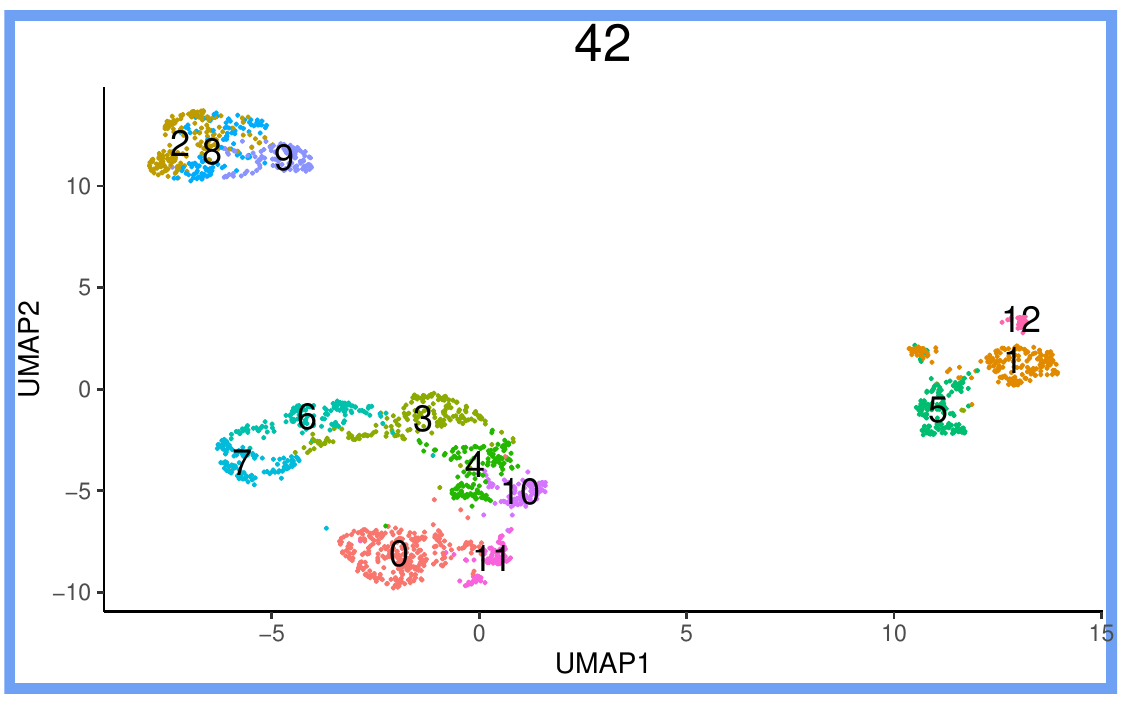
\includegraphics[width=7cm]{images/ch2/2_S1.png}
    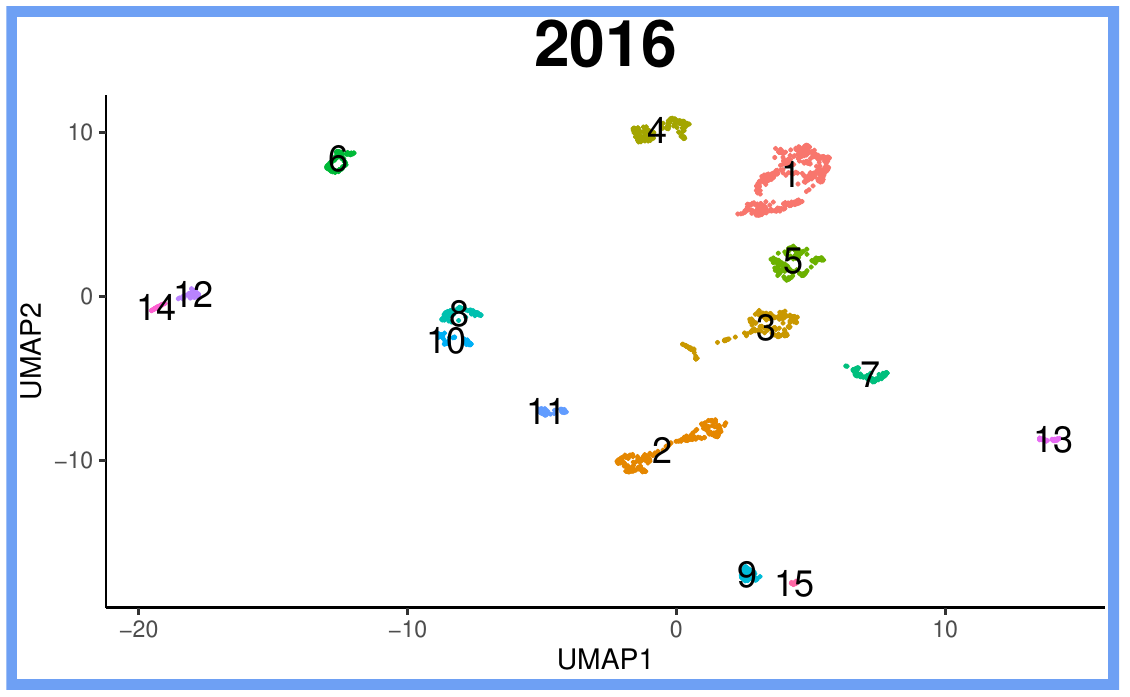
\includegraphics[width=7cm]{images/ch2/2_M1.png}
    \caption{\textbf{Results obtained on default results} Clustering distribution with default parameters for Monocle (right) and Seurat
(left). The title indicates the default random seed that is used.}
\end{figure}
\end{frame}

\begin{frame}{Aligning the results}
  \begin{table}[H]
    \resizebox{\textwidth}{!}{
    
            \begin{tabular}{|l|l|l|l|}
                \hline
                \textbf{Parameter name}     & \textbf{Step}                            & \textbf{Monocle value}    & \textbf{Seurat value}     \\ \hline
                \textbf{seed}               & \cellcolor[HTML]{6D9FF3}-                & 2016                      & 42                        \\ \hline
                \textbf{feature set}        & \cellcolor[HTML]{E7A101}Dim reduction    & all genes                 & HV genes                  \\ \hline
                \textbf{UMAP min dist}      & \cellcolor[HTML]{E7A101}Dim reduction    & 0.1                       & 0.3                       \\ \hline
                \textbf{UMAP n neighbours}  & \cellcolor[HTML]{E7A101}Dim reduction    & 15                        & 30                        \\ \hline
                \textbf{base embedding}     & \cellcolor[HTML]{BE809D}Graph building   & UMAP                      & PCA                       \\ \hline
                \textbf{SNN implementation} & \cellcolor[HTML]{BE809D}Graph building   & \begin{tabular}[c]{@{}l@{}}no self-neighbours\\ only direct neighbours\end{tabular} & \begin{tabular}[c]{@{}l@{}}with self-neighbours\\ direct and indirect neighbours\end{tabular} \\ \hline
                \textbf{graph type}         & \cellcolor[HTML]{BE809D}Graph building   & unweighted                & weighted                  \\ \hline
                \textbf{clustering method}  & \cellcolor[HTML]{72B980}Graph clustering & Leiden                    & Louvain                   \\ \hline
                \textbf{quality function}   & \cellcolor[HTML]{72B980}Graph clustering & CPM                       & RBConfiguration           \\ \hline
                \textbf{resolution}         & \cellcolor[HTML]{72B980}Graph clustering & 1e-4                      & 0.8                       \\ \hline
                \textbf{\#iterations}       & \cellcolor[HTML]{72B980}Graph clustering & 2                         & 10                        \\ \hline
            \end{tabular}}
            \caption{\textbf{Parameters used for aligning the results of the two packages}}
        \end{table}
    

\end{frame}
\section{ClustAssess package}

\subsection{ECS optimization}

\begin{frame}[label=ecs-first]{What is ECS?}
    \begin{itemize}[<+->]
        \item An \textit{affinity matrix} of a partition describe the co-occurrences of different elements by calculating the number of different paths between them.
        \item  For a disjoint partition, the affinity matrix can be calculated using the formula: \begin{equation*} \label{eq:affinity-disjoin}
                  p_{ij} =
                  \begin{cases}
                      0, \text{if } i \text{ and } j \text{ don't belong to the same cluster}                  \\
                      \frac{\alpha}{|C_\beta|}, \text{if }i\text{ and } j \text{ belong to the cluster } \beta \\
                      1 - \alpha + \frac{\alpha}{|C_\beta|}, \text{if } i = j
                  \end{cases}
              \end{equation*}
        \item Element-Centric Similarity (ECS) \cite{Gates2019} is a clustering comparison score measured using the L1 distance between the affinity matrices: $ \displaystyle S_i (\mathcal{A}, \mathcal{B}) = 1 - \frac{1}{2 \alpha} \sum_{j = 1}^N |p_{ij}^{\mathcal{A}} - p_{ij}^{\mathcal{B}}|$
    \end{itemize}

    \hyperlink{app1}{\beamerbutton{ECS properties}}

\end{frame}

\begin{frame}{Optimising the calculation of the ECS score for disjoint partitions}
    \begin{itemize}
        \item For disjoint partitions, the ECS has the same value for points from the same clusters.
        \item The number of ECS calculations drops from $N \times N$ to $n \times m$.
        \item This optimization removes the affinity matrix dependency and should be both time and memory efficient.

    \end{itemize}
\end{frame}

\begin{frame}{Element-Centric Consistency}
    \begin{itemize}
        \item Gates et al. also proposed Element-Centric Consistency (or ECC; also named  \textit{frustration}) score, used when a list of multiple partitions is provided.
        \item The ECC score is calculated as the average of the sum of the ECS between every unique pair of partitions from the list:
              \begin{equation*}
                  \frac{2}{T(T-1)} \sum_{j=1}^T \sum_{k=1}^{j-1} S_i (\mathcal{R}_k, \mathcal{R}_j)
              \end{equation*}
    \end{itemize}
\end{frame}


\begin{frame}[label=wecc]{Weighted ECC}
    \begin{itemize}
        \item If there are multiple occurrences of the same partition, determining the ECC will require rendundant calculation of the ECS of the same pairs.
        \item To prevent this, we propose a weighted version of ECC, where each unique partition has attached a weight that denotes the number of duplicates.
    \end{itemize}
    \hyperlink{weight-ecc}{\beamerbutton{Weighted ECC pseudocode}}
\end{frame}

\begin{frame}{Merging identical partitions}
    \begin{columns}
        \begin{column}{0.45\textwidth}
            \justifying

            The weights are calculated by performing an automatic merge of identical partitions.
            \bigskip

            To determine if two partitions are identical, we use their contingency table.
        \end{column}

        \begin{column}{0.5\textwidth}
            \begin{figure}
                \centering
                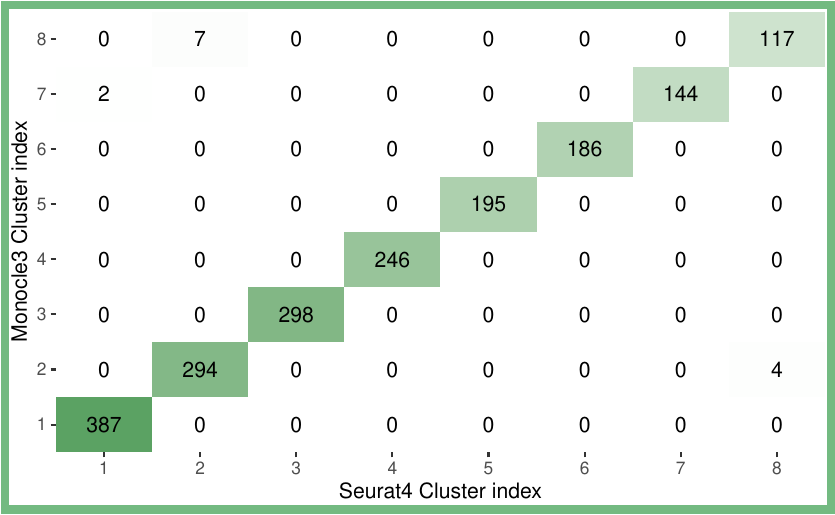
\includegraphics[width=\textwidth]{images/ch2/2_cont_table.png}
                \caption{\justifying \textbf{Contingency table}. The rows are associated with the clusters from one partition, and the columns with the clusters from the other partitions. }
            \end{figure}
        \end{column}
    \end{columns}
    
\end{frame}
\begin{frame}{Almost identical partitions - ECS threshold}
    There can be cases where the difference between two partitions is negligible, as it can be seen in the picture below.
    To allow the merge of almost identical partitions, we introduced the \textit{ECS threhshold}: the value of this parameter acts as a lower bound and determines whether the partitions should be considered extremely similar and mergeable or not.
    \begin{figure}
        \centering
        \begin{subfigure}[t]{0.47\textwidth}
            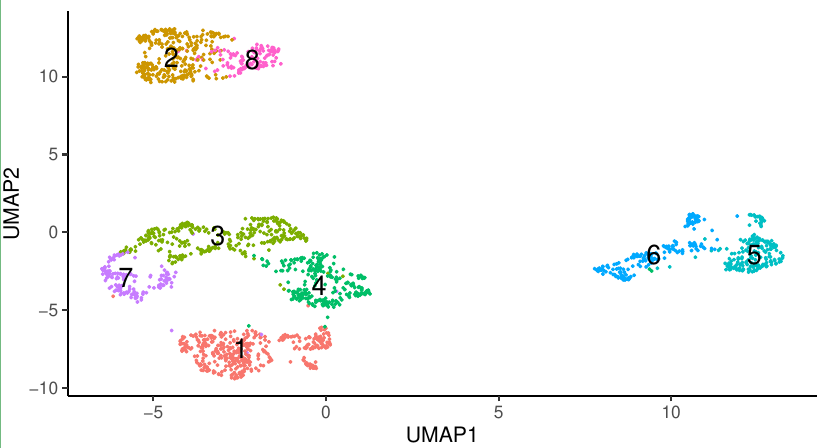
\includegraphics[width=\textwidth]{images/ch2/2_almost_s.png}
        \end{subfigure}
        \begin{subfigure}[b]{0.47\textwidth}
            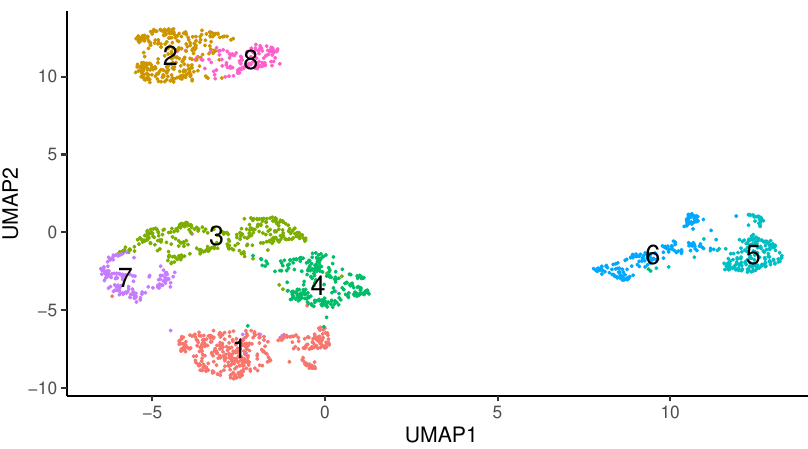
\includegraphics[width=\textwidth]{images/ch2/2_almost_m.png}
        \end{subfigure}
        \caption{\textbf{Two almost identical partitions} Each panel represents the distribution of a partition on a low-dimensional (UMAP) topology.}
    \end{figure}
\end{frame}

\subsection{Stability pipeline}

\begin{frame}
    \begin{itemize}
        \item Random seed is a factor that affects the clustering output.
        \item We developed a stability pipeline that performs a visual assessment of the robustness of a parameter configuration at the change of seed.
        \item The robustness will be determined by running the clustering pipeline multiple times with different random seeds. The Element-Centric Consistency of the obtained list of partitions will be an indicator of stability.
        \item The stability pipeline follows the steps presented in the PhenoGraph algorithm.
    \end{itemize}
\end{frame}

\begin{frame}{Feature stability}
    \begin{columns}
        \begin{column}{0.45\textwidth}
            \justifying

            The feature set has an important role in obtaining the low-dimensional topology.
            \bigskip


            We can assess the stability of different feature sets with varying sizes.
            \bigskip


        \end{column}

        \begin{column}{0.5\textwidth}
            \begin{figure}
                \centering
                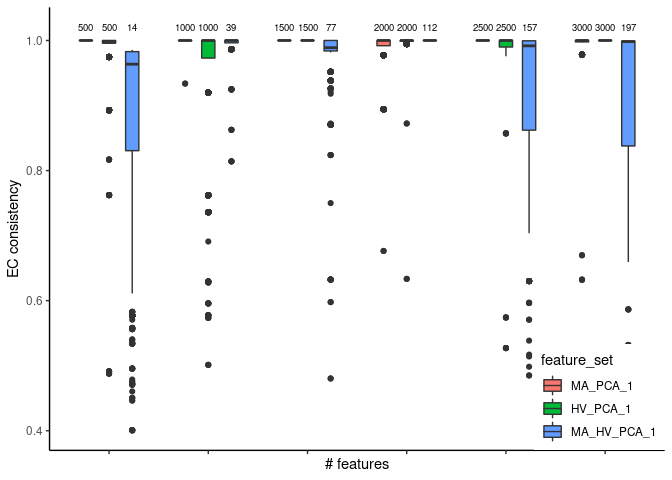
\includegraphics[width=\textwidth]{images/ch3/3_feat_incremental.png}
                \caption{\justifying \textbf{Incremental feature stability}. Each colour represents a different feature set. The size of the set is displayed above each boxplot. Each boxplot represents the consistency of the partitions. }
            \end{figure}
        \end{column}
    \end{columns}
\end{frame}

\begin{frame}{Inference of minimum number of clusters}
    \begin{columns}
        \begin{column}{0.45\textwidth}
            \justifying

            The number of nearest neighbours affect the graph connectivity.
            \bigskip


            The number of connected components decreases as the number of nearest neighbours increases.
            \bigskip

            The number of connected components acts as a lower bound for the possible number of clusters.


        \end{column}

        \begin{column}{0.5\textwidth}
            \begin{figure}
                \centering
                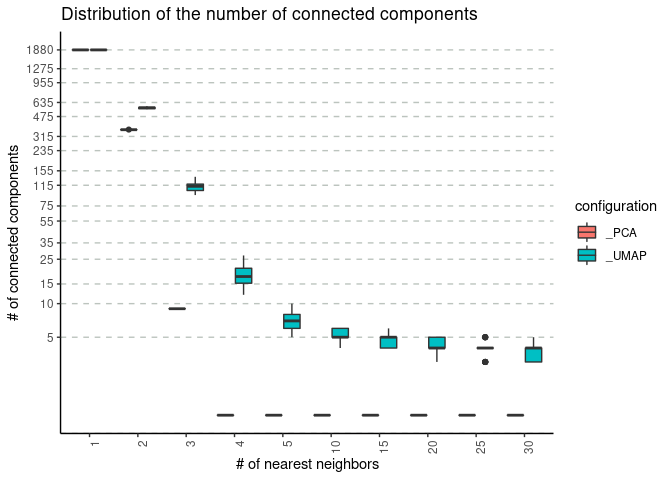
\includegraphics[width=\textwidth]{images/ch3/3_conn_comp.png}
                \caption{\justifying \textbf{Graph connectivity evolution}. Each colour represents a different reduced space used for graph building. The X-axis represents the number of nearest neighbours used. The Y-axis represents the number of connected components. }
            \end{figure}
        \end{column}
    \end{columns}
\end{frame}


\begin{frame}{Resolution - number of clusters stability}
    \begin{columns}
        \begin{column}{0.45\textwidth}
            \justifying

            For graph clustering methods, the resolution parameter controls the number of clusters.
            \bigskip


            The stability can be assessed on different parameter configurations.
            \bigskip

            The colour gradient describes the statistical reliability of the assessment.


        \end{column}

        \begin{column}{0.5\textwidth}
            \begin{figure}
                \centering
                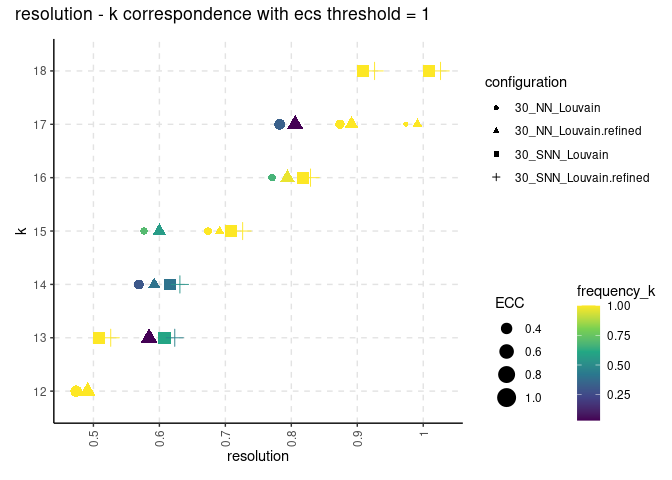
\includegraphics[width=\textwidth]{images/ch3/3_1_kres_ecc.png}
                \caption{\justifying \textbf{Resolution - number of cluster stability}. Each shape of point indicate a different parameter configuration. The point size indicates the stability of the resolution - number of clusters pair. The colour gradient illustrates the frequency of the number of clusters.}
            \end{figure}
        \end{column}
    \end{columns}
\end{frame}
\section{Benchmark results}

\subsection{ClustAssess vs Clusim - ECS benchmarks}

\begin{frame}
    \begin{itemize}[<+->]
        \item To benchmark the performance of the \texttt{ClustAssess} package, we compare it to \texttt{Clusim}. 
        \item \texttt{Clusim} is a Python package that contains the official implementation from the authors of the ECS paper \cite{Gates2019b}.
        \item In \texttt{Clusim}, the ECS between two disjoint partitions is determined based on the affinity matrices.
        \item The benchmark relies on the ECS between two fixed partitions using the implementations from \texttt{ClustAssess} and \texttt{Clusim}. The size of the partitions varies from 50 to 90 000. The number of clusters is set to 20 for both partitions. The assessment is repeated 30 times.
    \end{itemize}
\end{frame}

\begin{frame}{Runtime comparison}
    \begin{columns}
        \begin{column}{0.45\textwidth}
            \justifying
           

           \texttt{ClustAssess} requires less than a second to calculate the ECS, while the execution time of \texttt{Clusim} increases exponentially.
        \end{column}

        \begin{column}{0.5\textwidth}
            \begin{figure}
                % \centering
                % \makebox[\textwidth][c]{
                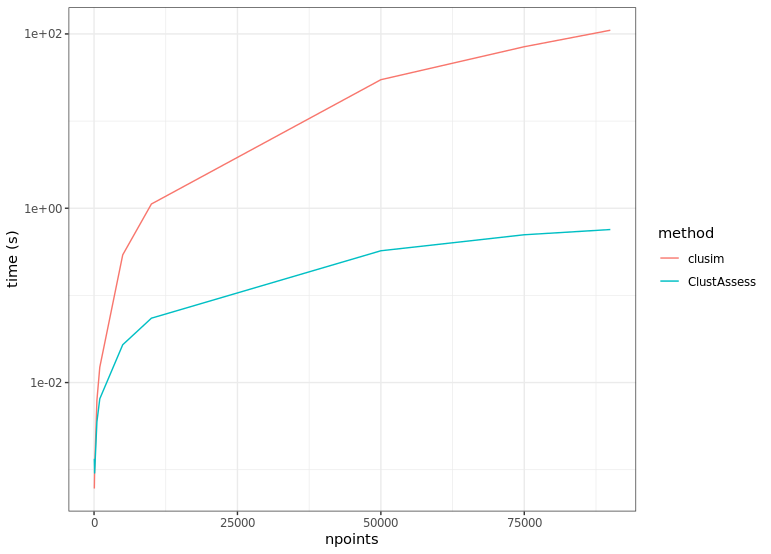
\includegraphics[width=0.95\textwidth]{images/ch4/4_clusim_ca_time.png}
                % }
                
                \caption{\justifying \textbf{Execution time benchmark} The size of the partitions used for the benchmark are displayed on the X-axis. The time (in seconds) required to calculate the ECS using ClustAssess (blue) and Clusim (red) is displayed on the Y-axis. The results are displayed on a logarithmic scale.}

            \end{figure}
        \end{column}
    \end{columns}
\end{frame}

\begin{frame}{Comparison of memory usage}
    \begin{columns}
        \begin{column}{0.45\textwidth}
            \justifying
            % The experiment was repeated to evaluate the memory required by each package to perform the calculation.

            For the optimized version from \texttt{ClustAssess} the data storage scales proportionally to the number of clusters. 
            \bigskip
            
           Memory allocation of $\leq$ 100 MiBs. 
           \bigskip

           The storage of the whole affinity matrix in \texttt{Clusim} is inefficient, reaching a memory allocation of 241 GiBs for the largest dataset.
        \end{column}

        \begin{column}{0.5\textwidth}
            \begin{figure}
                % \centering
                % \makebox[\textwidth][c]{
                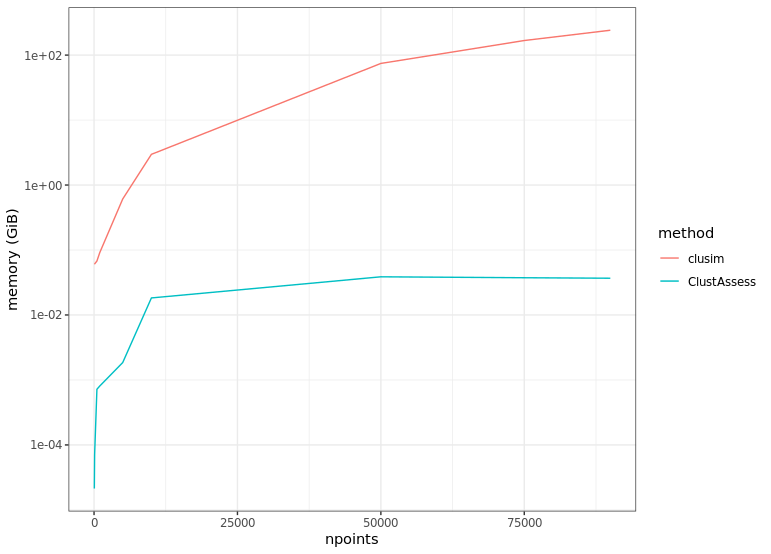
\includegraphics[width=0.95\textwidth]{images/ch4/4_clusim_ca_memory.png}
                % }
                \caption{\justifying \textbf{Memory usage benchmark} The size of the partitions used for the benchmark are displayed on the X-axis. The amount of memory (in GiBs) required to calculate the ECS using ClustAssess (blue) and Clusim (red) is displayed on the Y-axis. The results are displayed on a logarithmic scale.}
            \end{figure}
        \end{column}
    \end{columns}
\end{frame}

\begin{frame}{Performance with varying number of clusters}
    \begin{itemize}
    \item The time complexity for calculating the ECS in \texttt{ClustAssess} is $O(nm)$, where $n$ and $m$ represent the number of clusters of both partitions.
        

    \item As the number of clusters increases, the \texttt{ClustAssess} package will require more time and space to calculate the ECS.

    \item \texttt{Clusim} calculates the whole affinity matrix, so its performance is not influenced by the number of clusters.

    \end{itemize}
\end{frame}

\begin{frame}{Performance with varying number of clusters}
    \begin{figure}
        \centering
        \begin{subfigure}[t]{0.47\textwidth}
            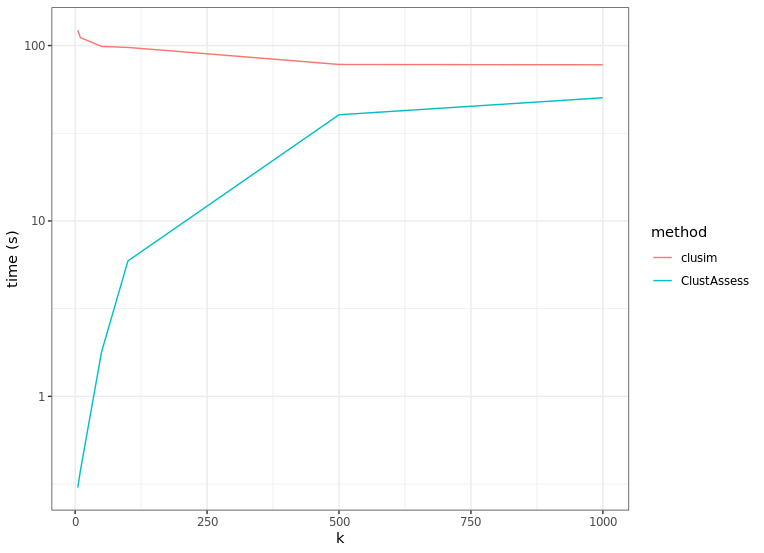
\includegraphics[width=\textwidth]{images/ch4/4_clusim_ca_time_k.png}
        \end{subfigure}
        \begin{subfigure}[b]{0.47\textwidth}
            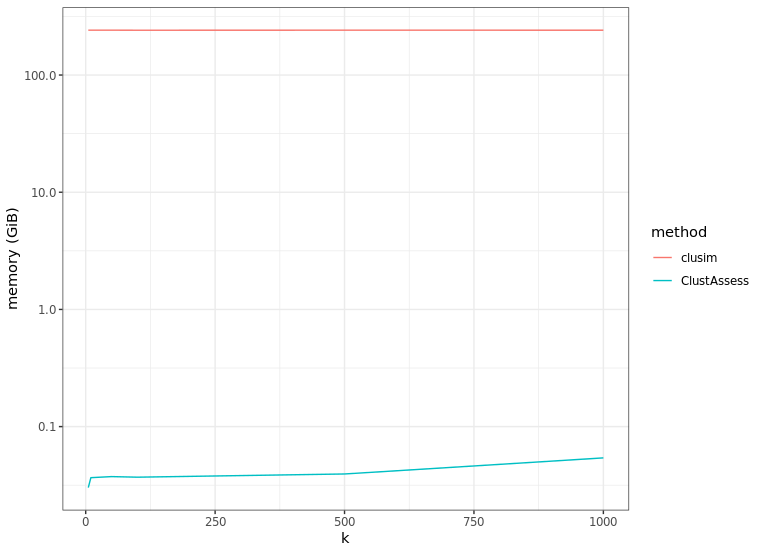
\includegraphics[width=\textwidth]{images/ch4/4_clusim_ca_memory_k.png}
        \end{subfigure}
        \caption{\textbf{Performance comparison for different number of clusters} Left panel - the median time of execution (in seconds) measured after 30 runs for ClustAssess (blue) and Clusim (red). Right panel - the median memory usage (in GiB) measured after 30 runs for ClustAssess (blue) and Clusim (red). The results are displayed on a linear scale.}
    \end{figure}
\end{frame}

\subsection{Stability pipeline benchmarks}

\begin{frame}{How the stability pipeline will be benchmarked}
    \begin{itemize}[<+->]
        \item We evaluated the performance of the five independent components: \texttt{feature\_stability}, \texttt{nn\_n\_conn\_comps}, \texttt{nn\_importance}, \texttt{clustering\_importance}, \texttt{resolution\_importance}.
        \item The stability pipeline was evaluated on the \textit{Mende et al} data \cite{Mende2022} with subsamples ranging from 1000 to 13000 cells.
        \item The pipeline allows support for parallelisation, i.e. we measured the pipeline's performance by varying the number of cores.
        \item We also evaluated the impact of using different ECS threshold values: 1, 0.99 and 0.95.
    \end{itemize}
\end{frame}

\begin{frame}
    \begin{figure}
                % \centering
                % \makebox[\textwidth][c]{
                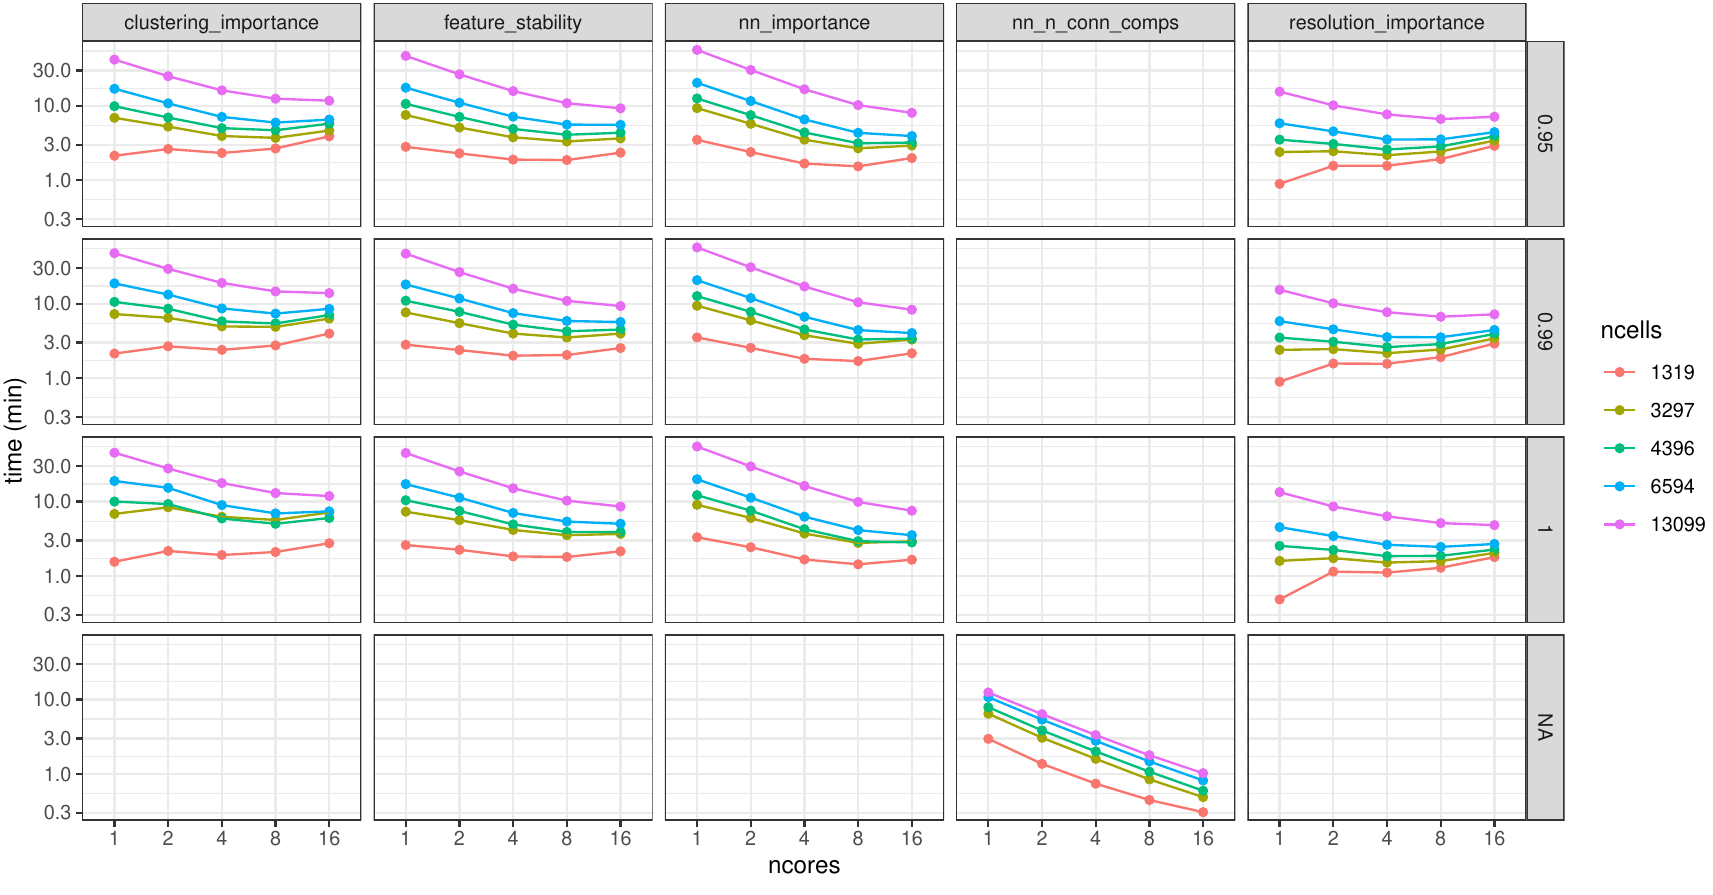
\includegraphics[width=0.8\textwidth]{images/ch4/4_pipeline.png}
                % }
                \caption{\justifying \textbf{Stability pipeline runtime benchmark} The columns correspond to different components of the pipeline. The rows indicate different ECS threshold values. On the X-axis we represent different number of cores. The Y-axis contains the runtime (in minutes). The colour indicates the size of the dataset.} %We observe no performance gain when ECS threshold is lowered. \texttt{nn\_n\_conn\_comps} has the best scaling when increasing the dataset, followed by \texttt{resolution\_importance}. Adding more cores generally brings a performance boost, with some exceptions related to the overhead created by either the small size of the dataset or the ratio between the number of runs and the number of cores. }
            \end{figure}
\end{frame}
\section{Acknwoledgements}

\begin{frame}{Acknwoledgements}
    The thesis is based on the ClustAssess paper to which I contributed as co-author.

    The paper was presented at CSCI 2022 annual retreat and will be presented at ECCB 2022.

    \begin{figure}
        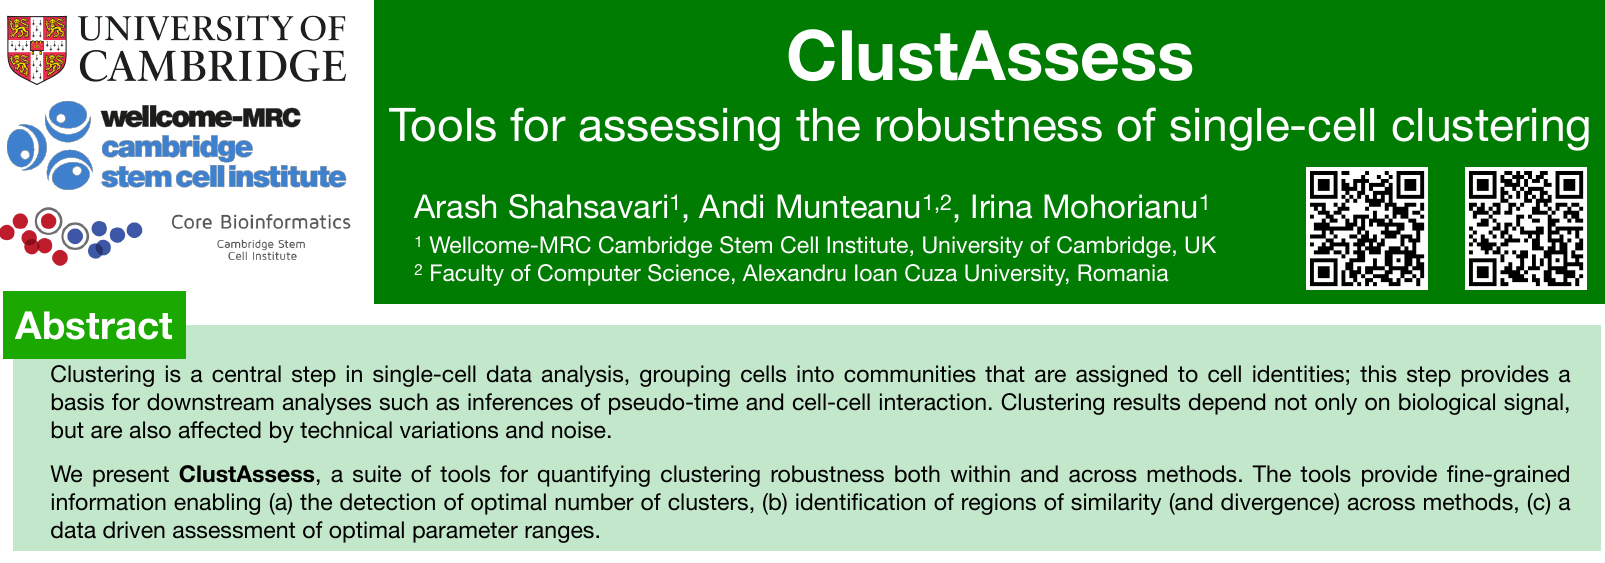
\includegraphics[width=\textwidth]{images/ca.png}
    \end{figure}
\end{frame}
% limiations and future work
\begin{frame}[allowframebreaks]{References}
\bibliographystyle{unsrt}
\bibliography{bibliography}
\end{frame}
\appendix

\begin{frame}[label=app1]{ECS properties}
    \hyperlink{ecs-first}{\beamergotobutton{Jump to ECS slide}}
\end{frame}

\begin{frame}[label=weight-ecc]{}
    \small
\begin{algorithm}[H]
    \SetKwInOut{Input}{input}\SetKwInOut{Output}{output}
    \SetKwInOut{Parameters}{parameters}
    \Input{$partList$: the list of disjoint partitions \\ $weights$: the weight array that contains the number of duplicates}
    \Output{the Element-Centric Consistency of the list}

    $nPartitions \gets \text{size}(partList)$; \\
    $nTotalPartitions \gets \text{sum}(weights)$; \tcp*{includes duplicates}
    $ecc \gets \textbf{0}$; \\
    % \tcp{Calculate the ECS between different partitions}
    \For{i = 1 \KwTo nPartitions - 1}{
        \For{j = i + 1 \KwTo nPartitions}{
            $ecc \gets ecc + \text{ecs}(partList[i],partList[j]) * weights[i] * weights[j];$
        }
    }
    
    % \tcp{Calculate the ECS between duplicates}
    $nDuplicatesECS \gets 0$; \\
    \For{i = 1 \KwTo nPartitions}{$nDuplicatesECS \gets nDuplicatesECS + weights[i] * (weights[i] - 1) / 2;$}
    $ecc \gets ecc + nDuplicatesECS * \textbf{1};$ \\
    % \tcp{Normalize the score in the range [0, 1]}
    $ecc \gets ecc / (nTotalPartitions * (nTotalPartitions - 1) / 2);$ \\
    \Return{ecc}

\end{algorithm}

\hyperlink{wecc}{\beamergotobutton{Jump to Weighted ECC slide}}

\end{frame}

\end{document}

